\clearpage
\newpage
\section{Figures}
\begin{figure}[H]
	\centering
	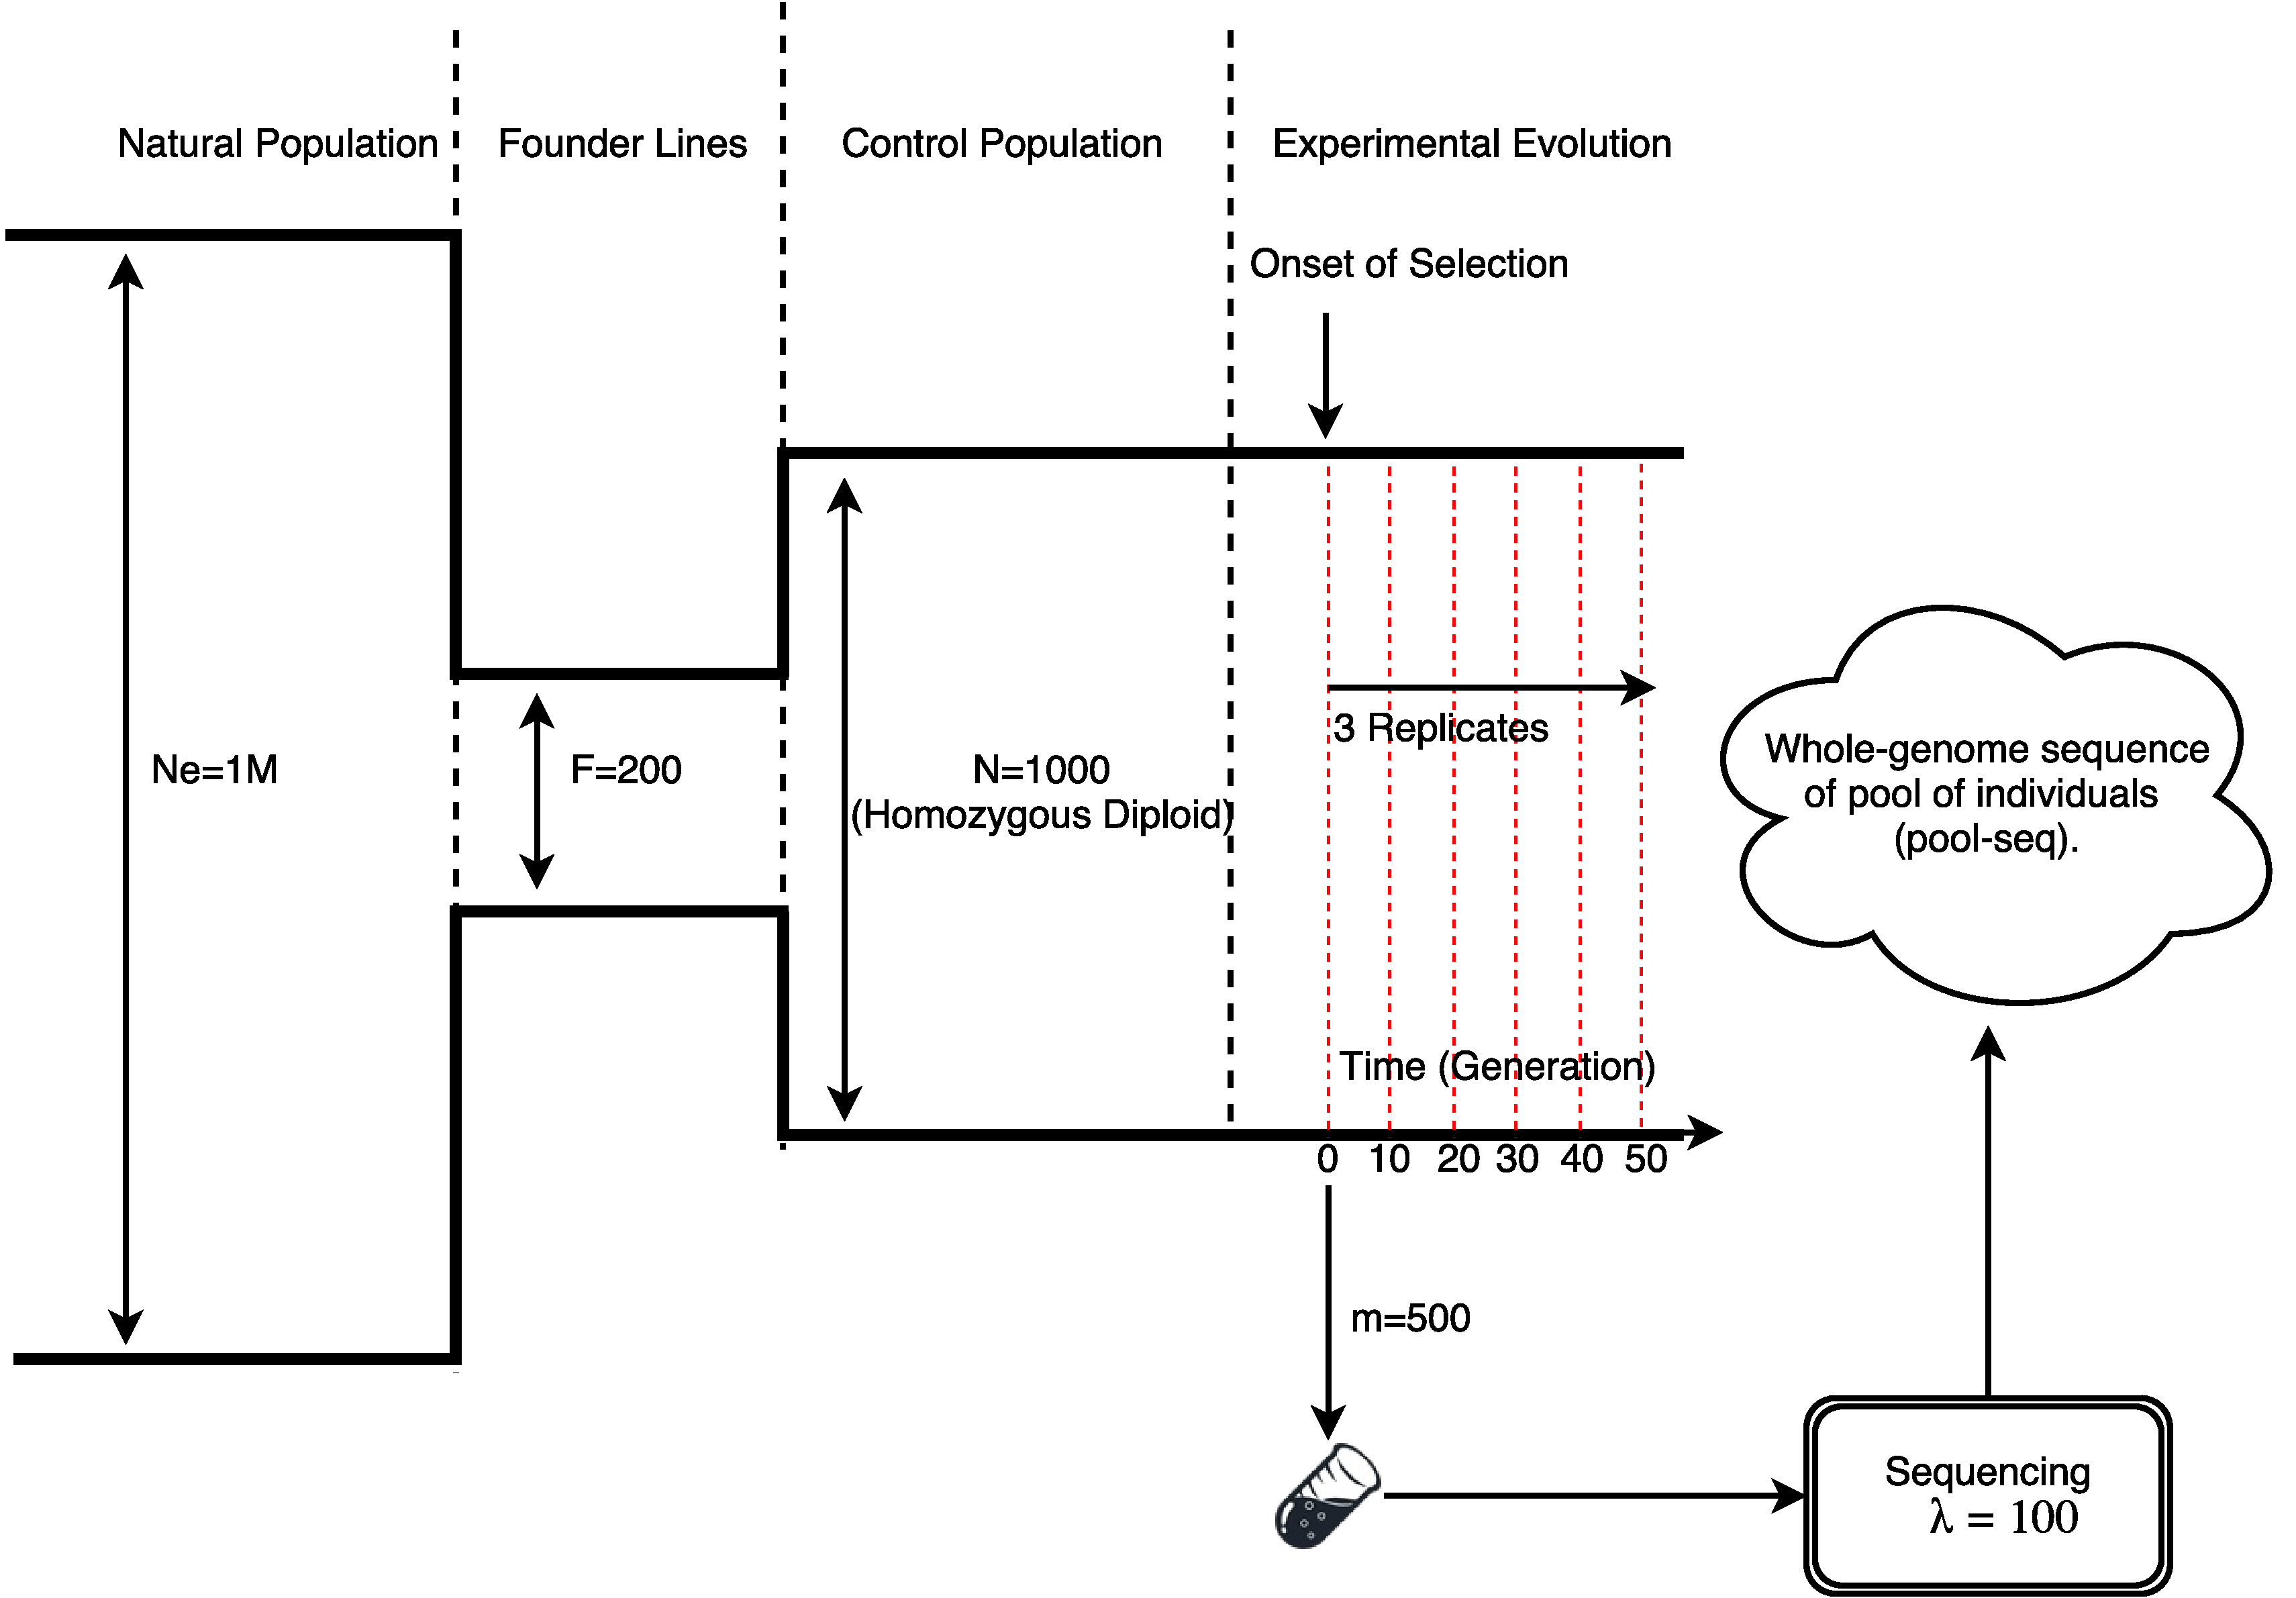
\includegraphics[trim=0.1in 0 .08in 0.02in , 
	clip,width=\textwidth]{figures/ExperimentalEvolution.pdf}
	\caption{ {\bf Two settings for collecting genomic time series
            data.}  Different settings in which dynamic data is
          collected are depicted with typical parameters for \emph{D.
            melanogaster}. In both settings, 6 samples (vertical red
          dashed lines) are taken every 10 generation.  When sampling
          from naturally evolving populations (A), the time of onset
          of selection is unknown, and population size is larger. For
          (controlled) experimental evolution, founder lines are first
          sampled from a natural population to create a homogeneous
          population. Multiple replicates of this population are
          evolved and sampled over time. }
	\label{fig:ee}
\end{figure}


\begin{figure}[H]
	\centering
	\includegraphics[width=\textwidth]{figures/{markovDists}.pdf}
        \caption{{\bf Comparison of empirical distributions of allele
            frequencies (green) versus predictions from Brownian
            Motion (red), and Markov chain (blue).} Panels A-F:
          Experiments were conducted under neutral evolution with
          different starting frequencies $\nu_0\in\{0.005,0.1\}$ and
          sampling times $\tau \in \{1,10,100\}$ generations. The
          empirical distribution was computed by sampling 143,900
          sites with $\nu_0=0.005$ and 47,500 variants with
          $\nu_0=0.1$. Panels G,H,I: Comparisons of Empirical and
          Markov chain based allele frequency distributions under a
          selection regime with $s=0.1$. Initial frequency was chosen
          as $\nu_0=0.005$ and sampling performed after $\tau$
          generations for $\tau \in \{1,10,100\}$.}
	\label{fig:markov}
\end{figure}

\begin{figure}[H]
	\centering
	\includegraphics[trim=.2in 0 .2in 0, 
	clip,width=\textwidth]{figures/{CLRQ}.pdf}
	\caption{{\bf Average power of composite statistics as function of 
	percentile cutoffs.} Detection power is averaged for 
	$s\in\{0.025,0.05,0.075,0.1\}$ using \comale statistic computed using 
	modified likelihood ration $\Hc(H)$ and standard likelihood ratio 
	$\Hc(|H|)$. For each setting the best performance is gained at  $\pi^*$ 
	which is different for different settings. As expected, $\pi^*$ takes 
	larger value (due to lower LD of the variation with favored allele). In 
	addition, for low coverage experiment better performance is achieved when 
	more candidate SNPs are take into computation of the composite statistic, 
	i.e., $\pi^*$ is lower. }
	\label{fig:clrq}
\end{figure}

\begin{figure}[H]
	\centering
	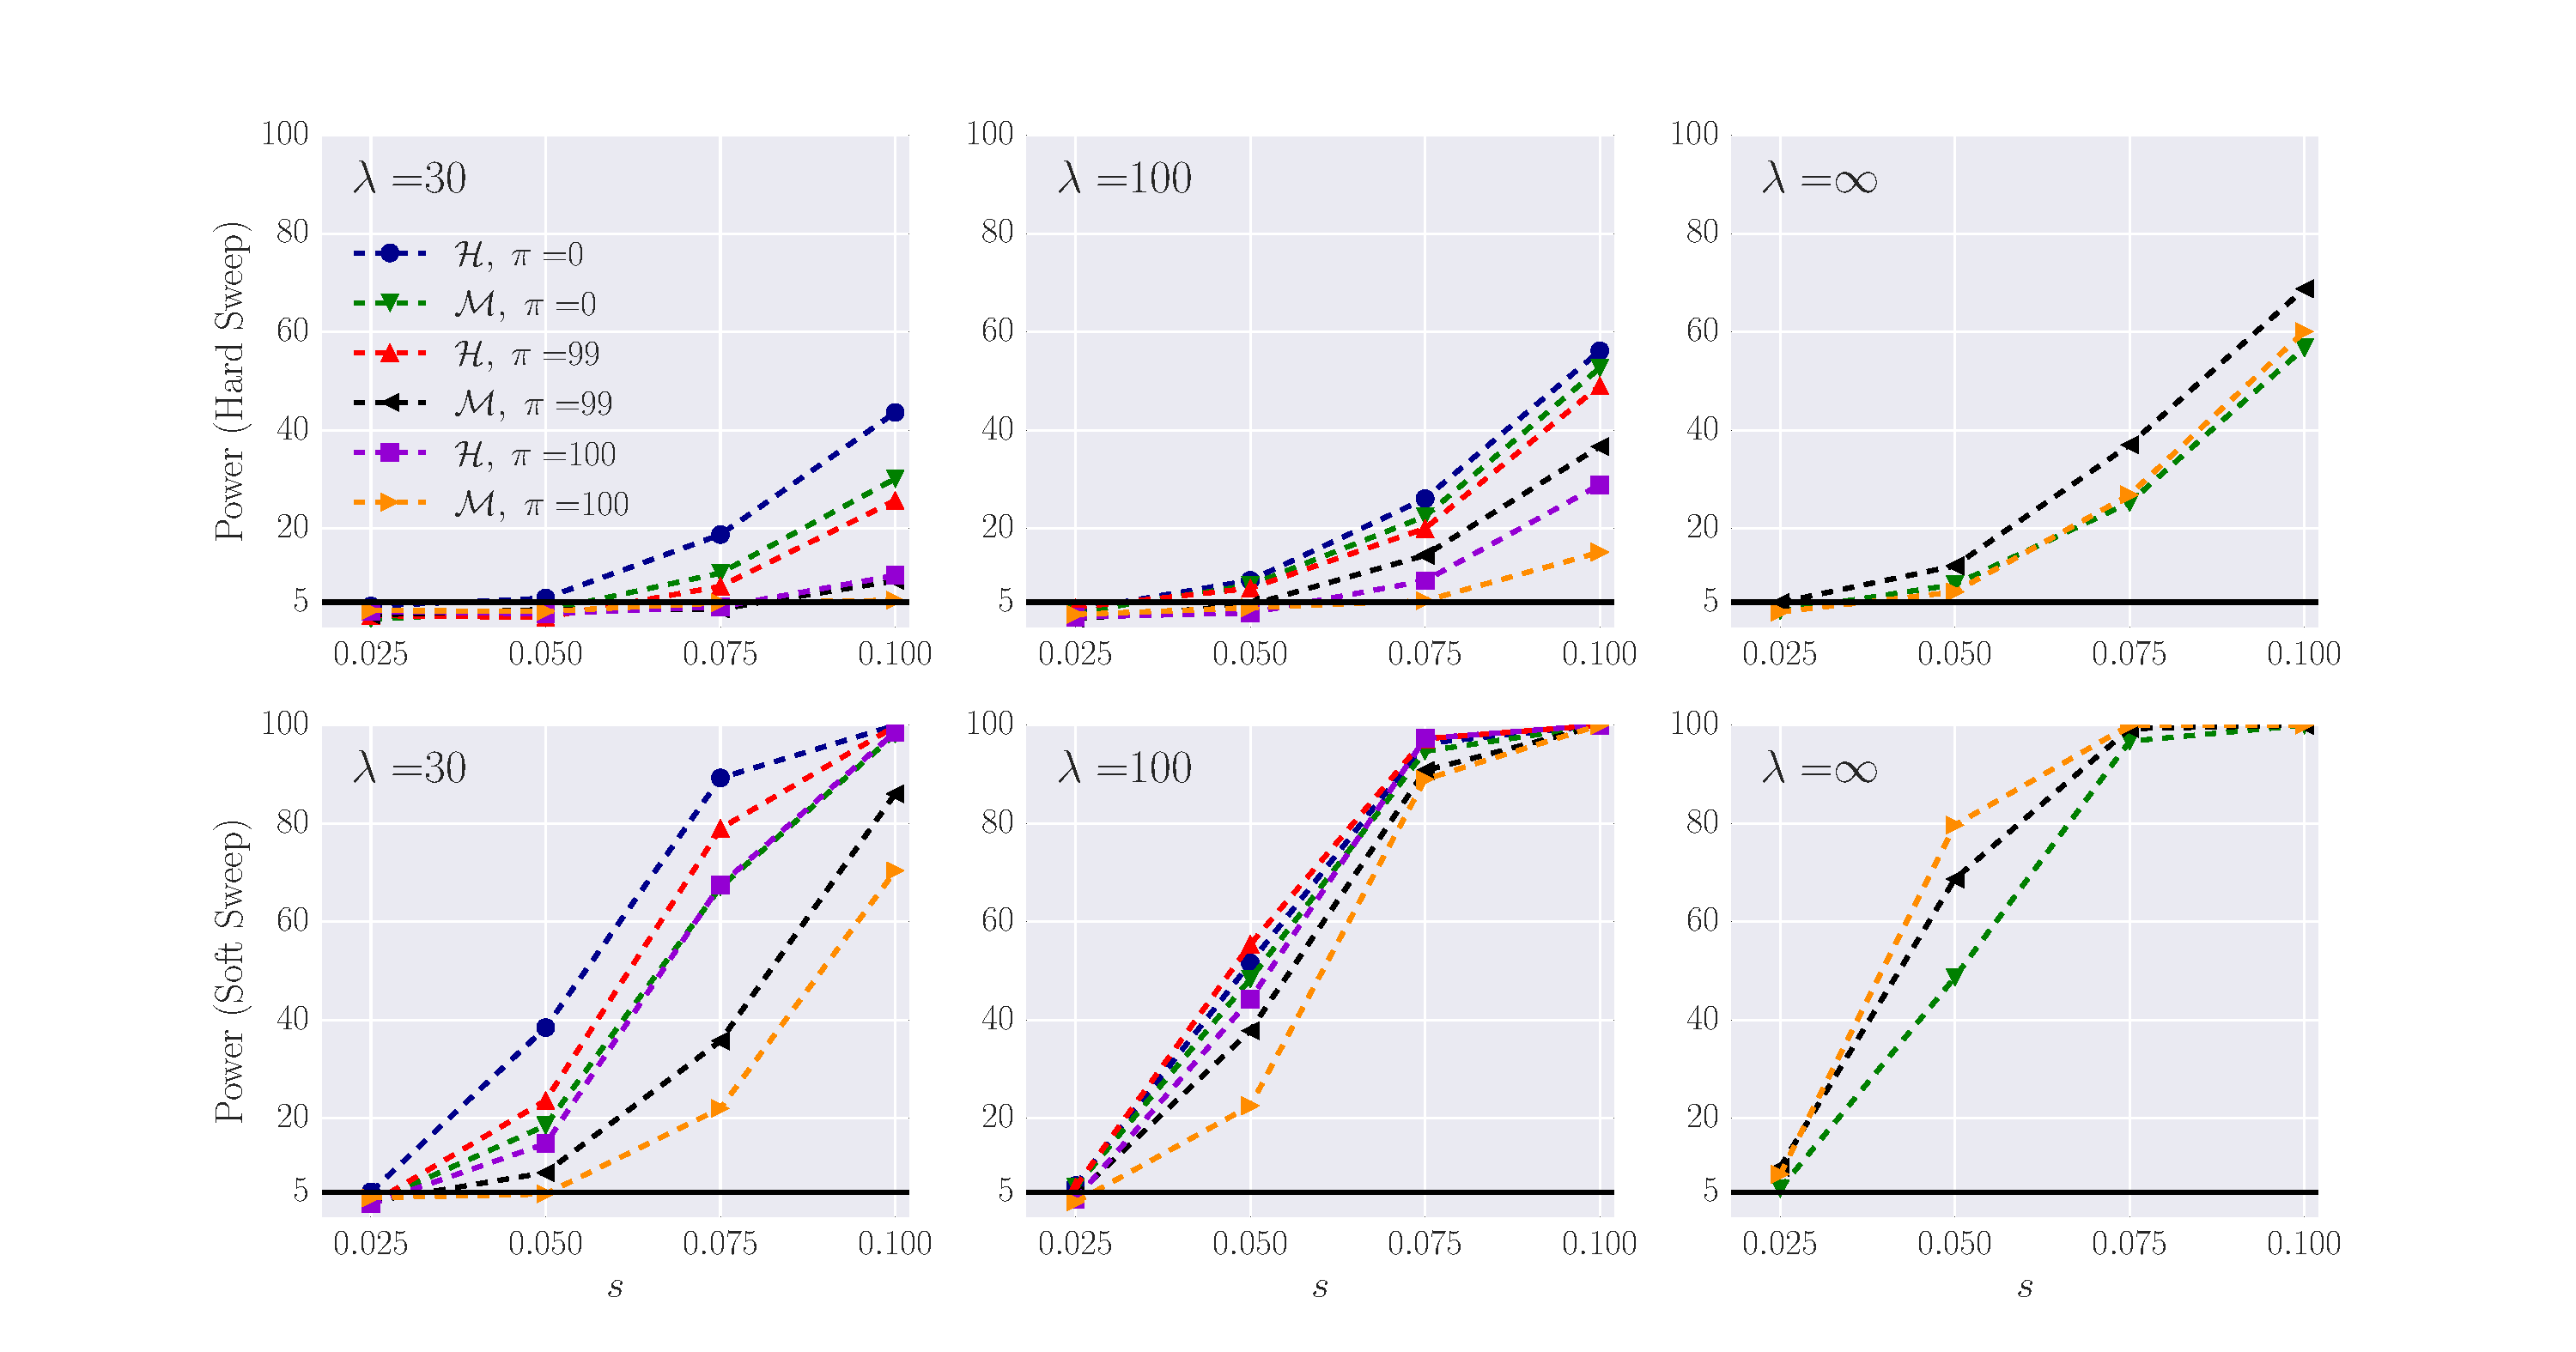
\includegraphics[width=\textwidth]{figures/powerCLR.pdf}
	\caption{{\bf Detection power of \comale-M and \comale-H with
            different composite statistics.}  Detection power for
          \comale-M ($\Mc$) and \comale-H ($\Hc$) under hard (top) and
          soft sweep (bottom) scenarios, for different settings of
          mean coverage $\lambda$ and selection strength $s$.  The
          $y$-axis measures power -- sensitivity with false positive
          rate FPR $\le 0.05$ -- for $1,000$ simulations of $50$Kbp
          regions.  } \label{fig:powerCLR}
\end{figure}

\begin{figure}[H]
	\centering
	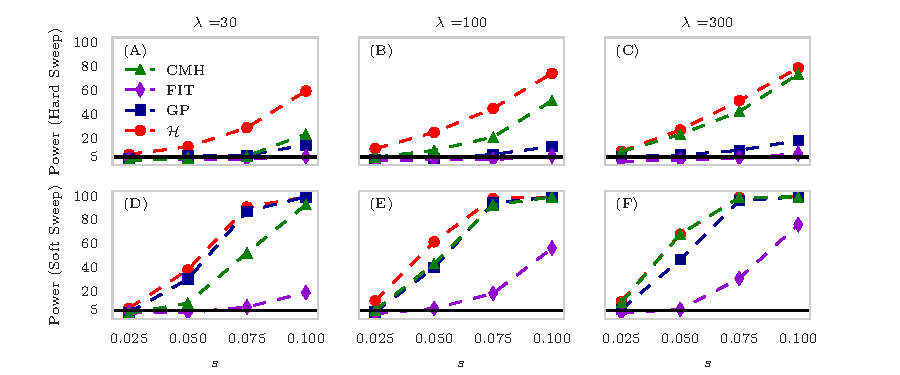
\includegraphics[width=\textwidth]{figures/power.pdf}
	\caption{ {\bf Power calculations for detection of selection.}
          Detection power for \comale ($\Hc$), Frequency Increment
          Test (FIT), Gaussian Process, and CMH under hard (top) and
          soft sweep (bottom) scenarios. $\lambda$, $s$ denote the
          mean coverage and selection coefficient, respectively. The
          $y$-axis measures power -- sensitivity with false positive
          rate FPR $\le 0.05$ -- for $1,000$ simulations of $50$Kbp
          regions. } \label{fig:power}
\end{figure}

\clearpage
\newpage
\begin{figure}[H]
	\centering
	\includegraphics[width=0.75\textwidth]{figures/{runTime.pdf}}
	\caption{{\bf Running time}. Box plot of running times
          (CPU-secs.) of \comale, HMM, GP with single, 3, 5, 7, and 10
          loci over 1000 simulations conducted on a workstation with
          4th Generation Intel Core i7 processor. The average running
          time for each method is shown on the x-axis.}
	\label{fig:runTime}
\end{figure}
\clearpage
\newpage

\begin{figure}[H]
	\centering
	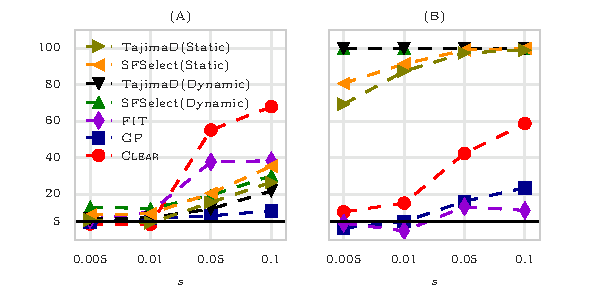
\includegraphics[width=0.7\textwidth]{figures/naturalee.pdf}
	\caption{{\bf Power of SFS based statistics.} Power of
          detecting selection for Frequency Increment Test (FIT),
          Gaussian Process (GP), \comale-H ($\Hc$) on hard-sweep
          natural experimental evolution with $N_e=10^4$ and depth
          $\lambda=\infty$. The measurements are conducted for a range
          of selection coefficients, $s$. Each point represents the
          mean of 200 simulations. For each simulation, sampling
          starts at a randomly chosen time, and subsequently 5
          replicate samples are acquired every $10$ generations.  (A)
          Start of sampling is chosen randomly throughout the sweep
          $\tau_1 \sim U\left[1,t_{\nu=1}(s,N_e)\right]$, where
          $t_{\nu=x}(s,N_e)$ denotes is the expected time to reach
          carrier frequency $x$ in a hard sweep and $U[a,b]$ is
          discrete uniform distribution. (B) The start of sampling is
          chosen near fixation of the favored allele, i.e. $\tau_1
          \sim
          U\left[t_{\nu=0.9}(s,N_e),t_{\nu=1}(s,N_e)\right]$.} 
          \label{fig:powerSFS}
\end{figure}

\clearpage
\newpage
\begin{figure}[H]
	\centering
	\includegraphics[trim=.2in 0 .2in 0, 
	clip,width=\textwidth]{figures/{rank100.0}.pdf}
	\caption{{\bf Ranking performance for 100X coverage.} Cumulative 
	Distribution Function (CDF) of the
          distribution of the rank of the adaptive allele in 500
          simulations for \comale-H, Gaussian Process (GP),
          CMH, and Frequency Increment Test (FIT), for different
          values of selection coefficient $s$ and initial carrier
          frequency. Area Under Curve (AUC) is computed as a
          quantitative measure ranking performance of methods for each
          configuration.}
	\label{fig:rank}
\end{figure}



\clearpage
\newpage
\begin{figure}[H]
	\centering
\includegraphics[width=0.7\textwidth]{figures/{bias.100}.pdf}
\caption{{\bf Distribution of bias for 100X coverage.} The
  distribution of bias ($s-\hat{s}$) in estimating selection
  coefficient over 500 simulations using Gaussian Process (GP) and
  \comale-H is shown for a range of choices for the selection
  coefficient $s$ and starting carrier frequency $\nu_0$, when
  coverage is 100.  The estimation performance of GP and HMM are very
  similar in soft sweep, while HMM provides lower variance in hard
  sweep(overall standard deviation is 0.036 for GO and is 0.028 for
  HMM).  }
	\label{fig:bias100}
\end{figure}

\clearpage
\newpage
\begin{figure}[H]
	\centering
	\includegraphics[width=\textwidth]{figures/{manhattan.min500snp}.pdf}
	\caption{{\bf \comale\ scan of the \data.}. Manhattan plot of the composite 
	$\Hc$
          statistic (A) and the number of SNPs (B) in 50Kbp
          sliding window with steps of 10Kbp, excluding windows close
          to centromere and telomere. The dashed line corresponds to
          the top $1$\%-ile cut-off and the candidate regions above the 
          threshold are show 
          in red dots. For comparison to past results,
          only Chromosomes 2, 3, and X are shown.}
	\label{fig:manhattancutoffed}
\end{figure}

\clearpage
\newpage